%\addcontentsline{toc}{chapter}{Annexe}
\chapter{Annexe}


\begin{figure}[!htb]
  \centering
  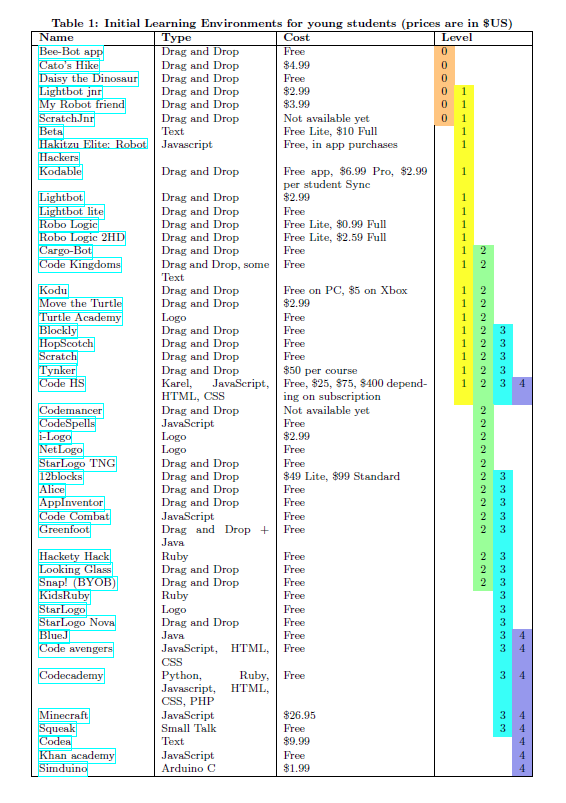
\includegraphics[width=150mm,scale=0.5]{initial_structure_env.PNG}
  \caption{Environnement de développement pour enfant, source : \cite{1}}
  \label{fig:boat1}
\end{figure}

\newpage

Tableau des primitives de Logo (Principales primitives de la tortue) :


\begin{table}[htb]
\begin{changemargin}{-3cm}{-3cm}
\begin{tabular}{|l|l|l|}
\hline
\multicolumn{1}{|c|}{Français} & Anglais            & Définition                                                                                         \\ \hline
AV n ou AVANCE n               & FD n ou Forward n  & La tortue avance de n pas                                                                          \\ \hline
RE n ou RECULE n               & BK n ou Back n     & La tortue recule de n pas                                                                          \\ \hline
TD n ou TOURNEDROITE n         & RT n ou RIGHT n    & La tortue tourne de n degrés d'angle vers la droite                                                \\ \hline
TG n ou TOURNEGAUCHE n         & LT n ou LEFT n     & La tortue tourne de n degrés d'angle vers la gauche                                                \\ \hline
LC ou LEVECRAYON               & PU or PENUP        & La tortue ne laisse pas de trace                                                                   \\ \hline
BC ou BAISSECRAYON             & PD or PENDOWN      & La tortue laisse sa trace (par défaut)                                                             \\ \hline
CT ou CACHETORTUE              & HT ou HIDETURTLE   & La tortue n'est plus visible sur l'écran graphique                                                 \\ \hline
MT ou MONTRETORTUE             & ST ou SHOWTURTLE   & La tortue est visible sur l'écran graphique                                                        \\ \hline
ENR ou ENROULE                 & WRAP               & Enroule l'écran graphique (valeur par défaut)                                                      \\ \hline
FEN                            & WINDOWS            & La tortue peut sortir du jardin et disparaître de l'écran graphique                                \\ \hline
CLOS                           & FENCE              & La tortue ne peut pas sortir du jardin                                                             \\ \hline
ORIGINE                        & HOME               & Retour au milieu du carré de salade                                                                \\ \hline
VE                             & CS ou CLEARSCREEN  & Efface toutes les traces et restaure l'état initial   \\ \hline
NETTOIE                        & CLEAN              & Efface toutes traces de l'écran graphique sans changer la position                    \\ \hline
VT                             & CT or CLEARTEXT    & Efface l'écran de commande                                                                         \\ \hline
FCC n                          & SETPC n            & Change la couleur du crayon, n est un entier positif                                               \\ \hline
FCFG n                         & SETBG n            & Change la couleur du fond, n est un entier positif                                                 \\ \hline
FCB n                          & *****              & Change la couleur des bords, n est un entier positif                                               \\ \hline
FCAP n                         & SETH ou SETHEADING & Fixe le cap de la tortue de manière absolue, selon l'angle de n degrés                             \\ \hline
FPOS {[}X Y{]}                 & SETPOS {[}X Y{]}   & Fixe la POSITION de la tortue avec une LISTE de 2 nombres entiers \\ \hline
CAP n                          & HEADING            & Retourne l'orientation de la tortue exprimée en degrés                                             \\ \hline
POSITION, POS                  & POS                & Retourne la position de la tortue en coordonnées cartésienn                                        \\ \hline
\end{tabular}
\end{changemargin}
\end{table}

\newpage 

Primitives Logo mathématiques :

\begin{table}[htb]
\begin{changemargin}{-3cm}{-3cm}
\begin{tabular}{|l|l|l|}
\hline
\multicolumn{1}{|c|}{Français} & Anglais         & Définition                                                            \\ \hline
n1 + n2                        & n1 + n2         & Addition de nombres réels - Ex : EC 45.124 + 11 ou EC (+ 45 10 78 23) \\ \hline
n1 - n2                        & n1 - n2         & Soustraction de nombres réels - Ex :EC 5 - 1.09                       \\ \hline
n1 * n2                        & n1 * n2         & Multiplication de nombres réels - Ex :EC 5 * 9                        \\ \hline
n1 / n2                        & n1 / n2         & Division de deux nombres réels - Ex :EC 45 / 9                        \\ \hline
SOMME n1 n2                    & SUM n1 n2       & Addition de nombres réels - Ex : EC SOMME 45 11                       \\ \hline
DIFF n1 n2                     & - n1 n2         & Soustraction de nombres réels - Ex :EC DIFF 5 1                       \\ \hline
PROD ou PRODUIT n1 n2          & PRODUCT n1 n2   & Multiplication de nombres réels - Ex :EC PROD 5 9.45                  \\ \hline
DIV n1 n2                      & QUOTIENT n1 n2  & Division de deux nombres réels - Ex :EC DIV 45 11                     \\ \hline
QUOTIENT n1 n2                 & QUOTIENT n1 n2  & Division de deux nombres réels - Ex :EC DIV 45 11                     \\ \hline
RESTE n1 n2                    & REMAINDER n1 n2 & Reste de la division                                                  \\ \hline
ENT n                          & INT n           & Renvoie la partie entière du nombre réel - Ex :EC ENT 55.75 -> 55      \\ \hline
ARRONDI n                      & ROUND n         & Arrondit un nombre réel - Ex :EC ARRONDI 55.75 -> 56                   \\ \hline
ABS n                          & ABS n           & Renvoie la valeur un nombre réel - Ex :EC ABS -55 -> 55                \\ \hline
HASARD n                       & RANDOM n        & Renvoie un nombre entier entre 0 et n-1                               \\ \hline
RC n ou racine n               & SQR n           & Renvoie la racine carré d'un nombre réel - Ex :EC RC 25 -> 5           \\ \hline
LOG n                          & LOG n           & Renvoie le logarithme naturel d'un réel                               \\ \hline
LOG10 n                        & LOG10 n         & Renvoie le logarithme de base 10 d'un réel                            \\ \hline
EXP n                          & EXP n           & Renvoie l'exponentielle d'un réel                                     \\ \hline
SIN n                          & SIN n           & Renvoie le sinus d'un réel n en degrés - Ex :SIN 30                   \\ \hline
COS n                          & COS n           & Renvoie le cosinus d'un réel n en degrés                              \\ \hline
TAN n                          & TAN n           & Renvoie la tangente d'un réel n en degrés                             \\ \hline
ATAN n                         & ATAN n          & Renvoie tangente d'arc d'un réel n en degrés                          \\ \hline
PI                             & PI              & 3.141592…                                                             \\ \hline
RADIANS n                      & RADIANS n       & Convertit un angle en radians n en degrés                             \\ \hline
DEGRES n                       & DEGRES n        & Convertit un angle en degrés n en radians                             \\ \hline
\end{tabular}
\end{changemargin}
\end{table}

\begin{figure}[!htb]
  \centering
  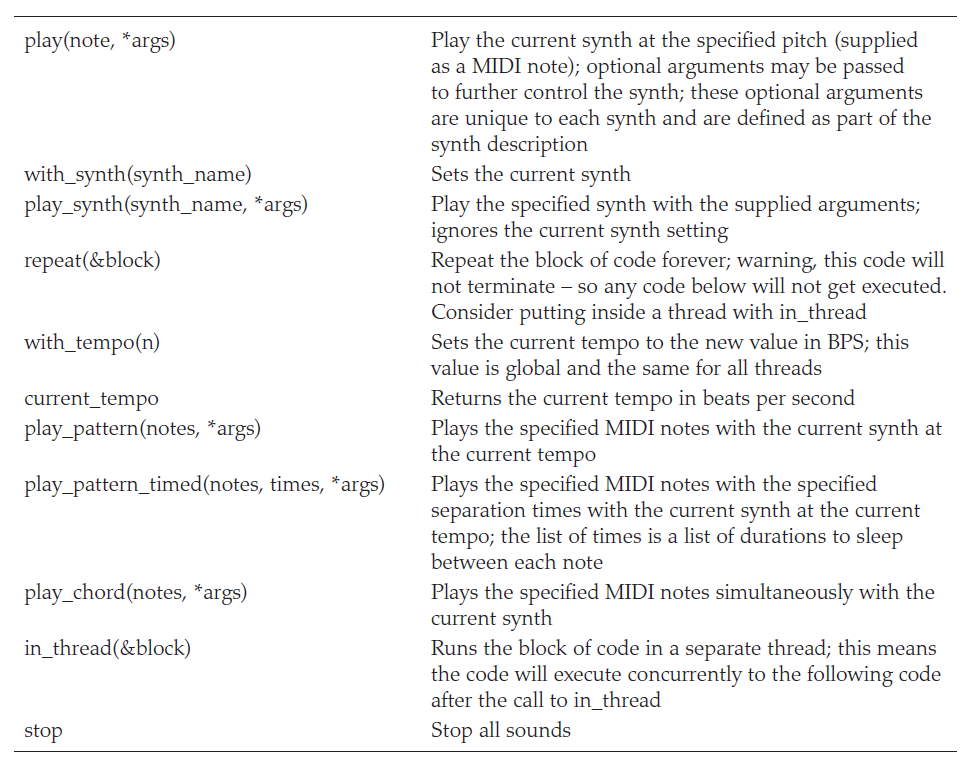
\includegraphics[width=105mm,scale=0.5]{images/sonic_pi_primitives.PNG}
  \caption{Exemples de fonctions de Sonic Pi, source : \cite{19}}
  \label{fig:boat1}
\end{figure}

\begin{lstlisting}[frame=single]

live_loop :beeps do
  start_note = ring(60, 62, 63, 62).tick
  my_chord = chord(start_note, :M7)
  play my_chord, release: 2
  16.times do
    play my_chord.choose, release: 0.25, amp: [0.75, 0.5, 0.25].choose
    sleep 0.125
  end
end

live_loop :drums do
  sample :loop_amen, beat_stretch: 2
  sleep 2
end

\end{lstlisting}

Exemple d'un programme Sonic Pi


\begin{figure}[!htb]
  \centering
  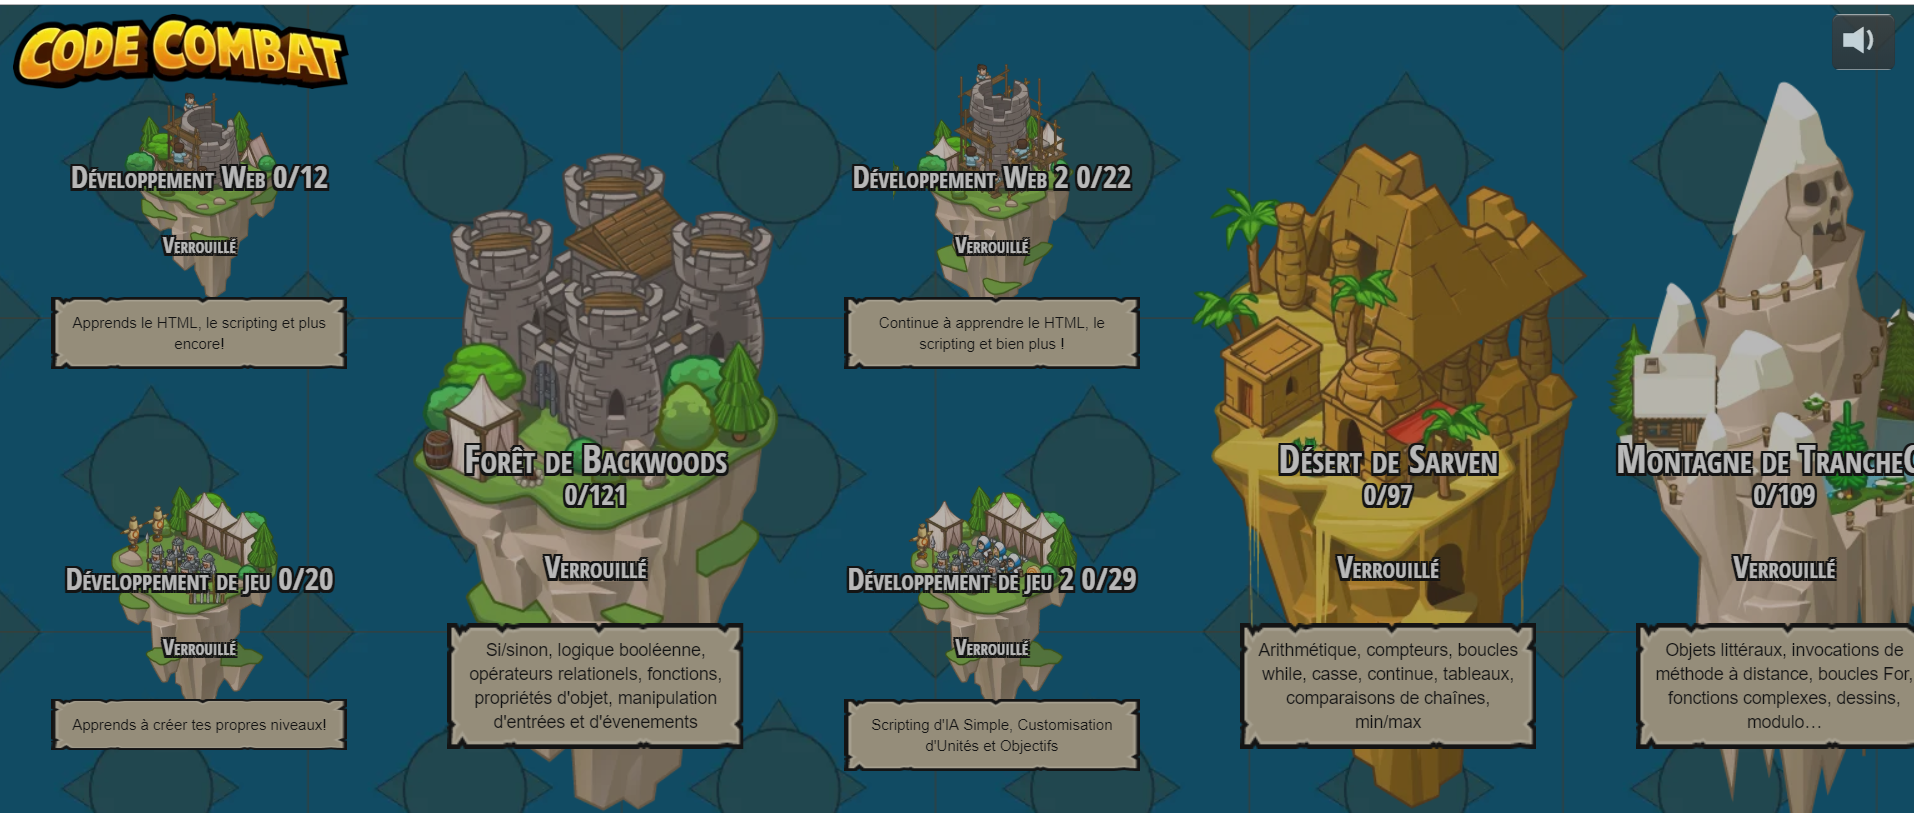
\includegraphics[height=80mm, width=150mm,scale=0.5]{images/codecombat3.PNG}
  \caption{Niveaux suivants de CodeCombat}
  \label{fig:boat1}
\end{figure}

\begin{figure}[!htb]
  \centering
  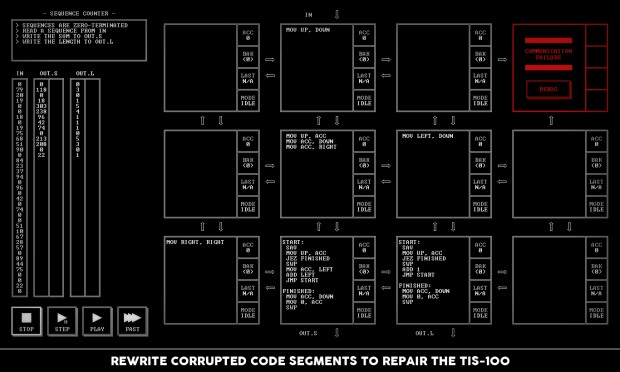
\includegraphics[width=150mm,scale=0.5]{images/tis-100.jpg}
  \caption{Interface TIS-100 et blocs de code}
  \label{fig:boat1}
\end{figure}

\begin{figure}[!htb]
  \centering
  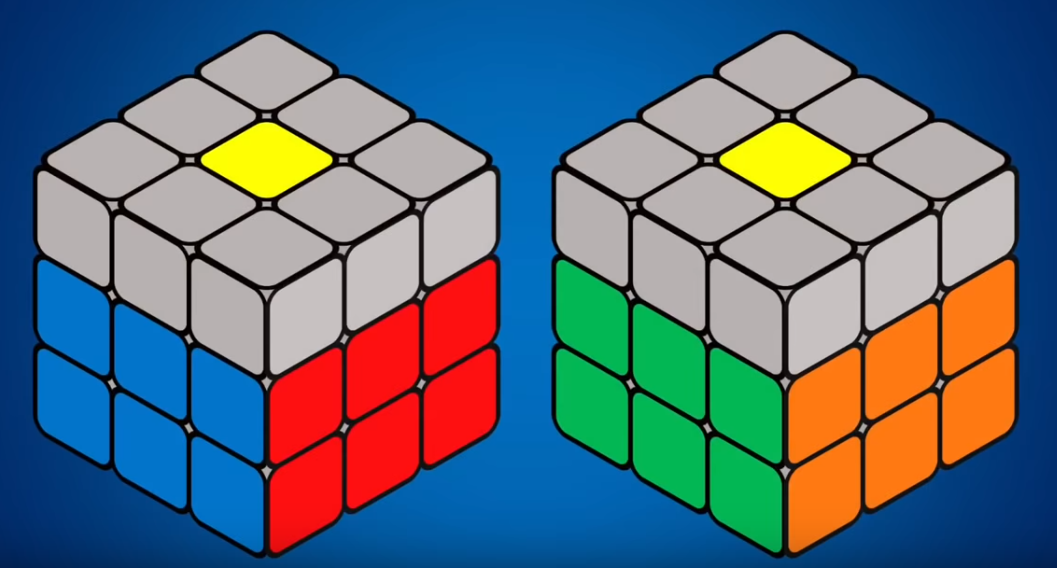
\includegraphics[width=80mm,scale=0.5]{images/rubiks-cube4.PNG}
  \caption{La deuxième couronne}
  \label{fig:boat1}
\end{figure}

\newpage

 
\newpage
Tous les algorithmes pour les étapes du Rubik's cube

\begin{lstlisting}[frame=single]

//face blanche
côté : d- b- d+ b+

//deuxième couronne
mettre à gauche : h- g- h+ g+ h+ a+ h- a-
mettre à droite : h+ d+ h- d- h- a- h+ a+
inversion : d+ h+ d- h2 d+ h2 d- h+ a- h- a+ 

//côté jaune après 2eme couronne
j jaune (1 en haut 1 à gauche) : d- h- a- h+ a+ d+
barre à l'horizontal : a+ d+ h+ d- h- a-
point jaune : d- h- a- h+ a+ d+ puis a+ d+ h+ d- h- a-

croix en face bien placé (2 bonne en face) : d+ h2 d- h- d+ h- d- puis
d+ h2 d- h- d+ h- d- h-

côté bien placé (mauvaise en face et à droite): d+ h2 d- h- d+ h- d- h-

1 coin à la bonne place + sens aiguille monte (le bon à droite) :
g- h+ d+ h- g+ h+ d- h-
coin à la bonne place 1 + sens inverse aiguille (le bon à gauche) : 
d+ h- g- h+ d- h- g+ h+
aucun bien placé : g- h+ d+ h- g+ h+ d- h-

-------------
coin bonne position 

2 mal orienté côte à côté (2pieces meme couleur à droite) : 
d+ h2 d- h- d+ h- d- g- h2 g+ h+ g- h+ g+
4 mal orienté (pareil à droite) : 
d+ h2 d- h- d+ h- d- g- h2 g+ h+ g- h+ g+
2 diagonale : a+ avec le jaune en face puis meme formule

3 coins mal orientés avec le jaune à droite : 
pareil avec 2 mauvais à droite
3 coins mal orientés avec le jaune à gauche : pareil

\end{lstlisting}

\newpage

\begin{figure}[!htb]
  \centering
  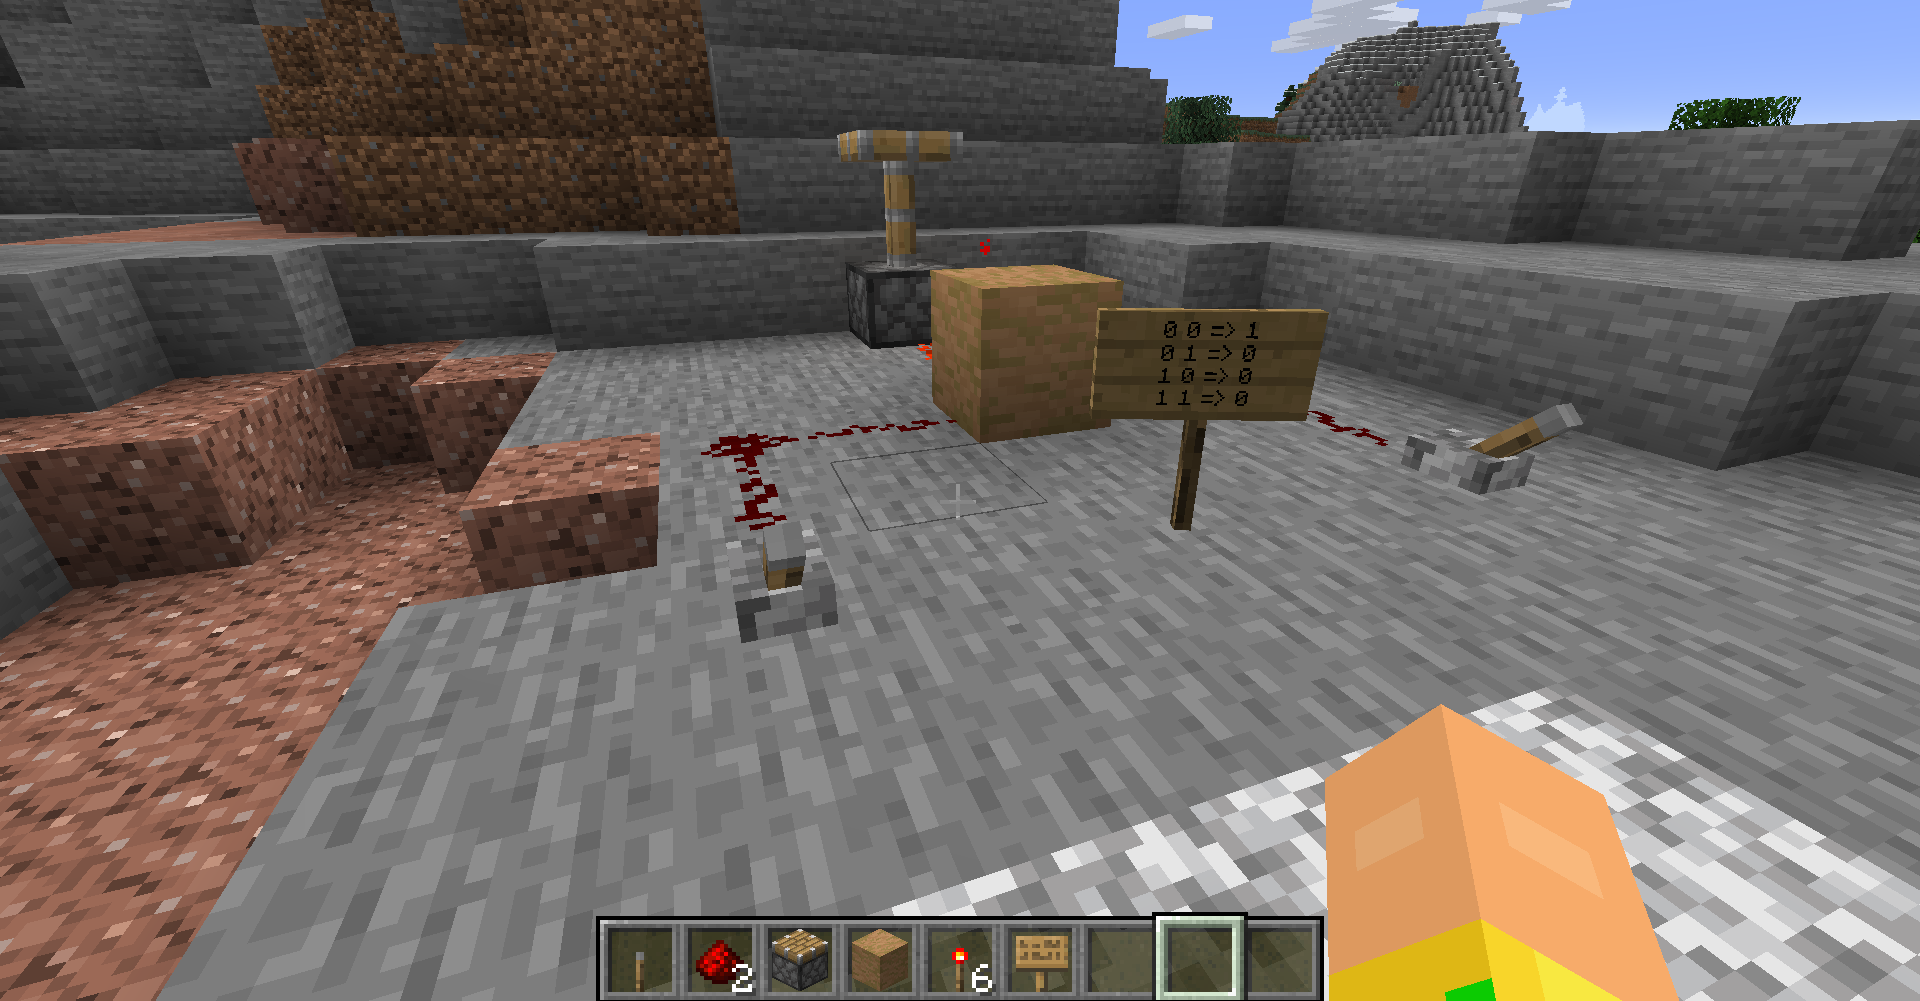
\includegraphics[width=120mm,scale=0.5]{images/minecraft6.png}
  \caption{Opérateur NOR dans minecraft}
  \label{fig:boat1}
\end{figure}

\begin{figure}[!htb]
  \centering
  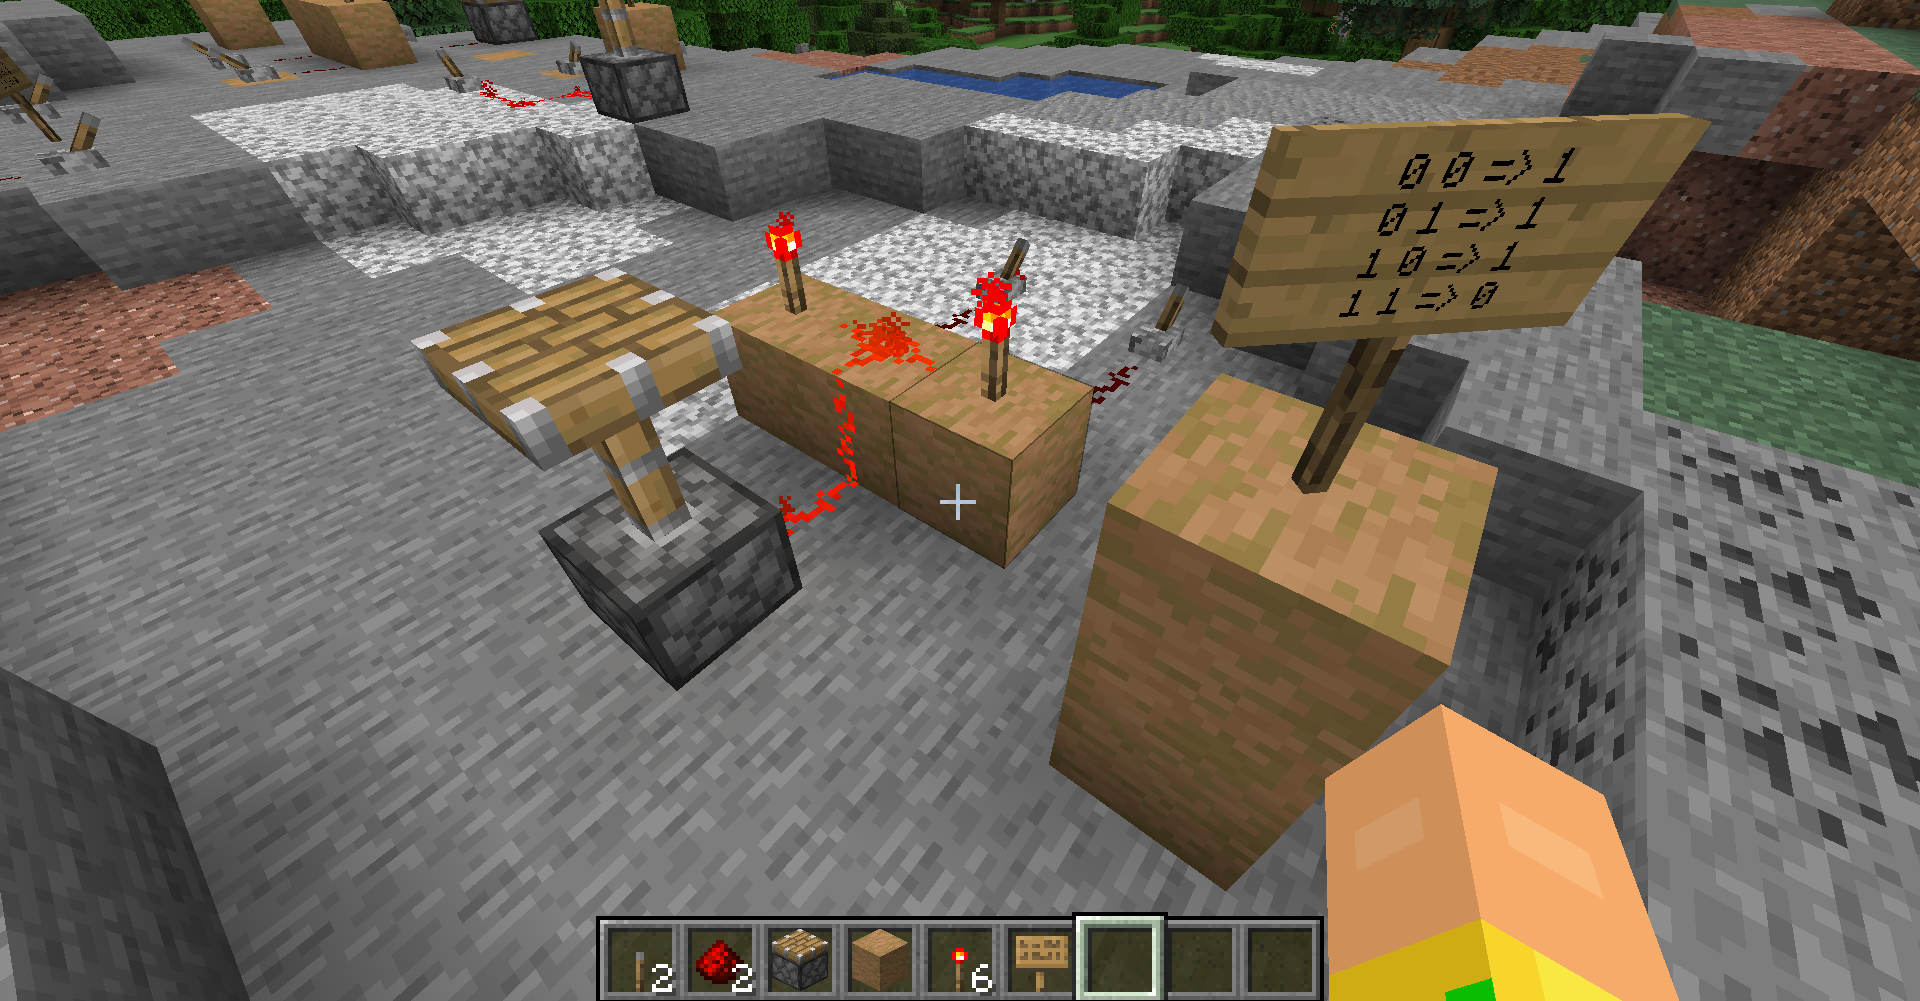
\includegraphics[width=120mm,scale=0.5]{images/minecraft7.png}
  \caption{Opérateur NAND dans minecraft}
  \label{fig:boat1}
\end{figure}